Jede Karte liefert eine spezielle Basis von $T_p \mfk$.

\begin{defs}
Sei $(x, U)$ eine Karte von $\mfk$ um $p$. 
Definiere Tangentialvektoren $\pdv{x_i} \eval_{p} $ ($i = 1, \dots, m$) wie folgt:
\begin{align}
\pdv{x_i}\eval_{p} (f) := \partial_i (f \circ x^{-1}) \eval_{x(p)}
\end{align}
Hierbei bedeutet $\partial_i$ die $i$-te partielle Ableitung.
\end{defs}

\begin{satz}
\label{satz:BasisTPM}
Die Tangentialvektoren $(\pdv{x_1}\eval_{p}, \dots, \pdv{x_m}\eval_{p})$ bilden eine Basis des $\tspace{p}$.
Jeder Tangentialvektor lässt sich schreiben als
\begin{align}
v = \sum_{i=1}^{m} v(x_i) \pdv{x_i}\eval_{p} = \sum_{i=1}^{m} \xi \pdv{x_i}\eval_{p}.
\end{align}
\end{satz}
\begin{bew}[Satz \ref{satz:BasisTPM} Teil 1]
Es gilt die lineare Unabhängigkeit:
\begin{align}
\pdv{x_i}\eval_{p} (x^j) = \delta_{i j}
\end{align}
Jetzt muss noch gezeigt werden, dass $(\pdv{x_1}\eval_{p}, \dots, \pdv{x_m}\eval_{p})$ ein Erzeugendensystem für $\tspace{p}$ ist.
 Dafür benötigen wir allerdings zunächst ein Hilfslemma.
\end{bew}

\begin{hlem}
\label{lem:DarstellungBasisTPM}
Sei $f: U \subset \mfk \to \R$ eine glatte Funktion.
Dann existiert eine Umgebung $U' \subset U$ von $p$ ($p \in U'$) und eine glatte Funktion
$f_i: U' \to \R$, so dass
\begin{align}
f = f(p) + \sum_{i=1}^{m} ( x_i  - x_i(p)) f_i.
\end{align}
Wobei $f_i (p) = \pdv{x_i}\eval_{p} (f)$.
\end{hlem}

\begin{bew} \leavevmode

\begin{figure}[H]
\centering
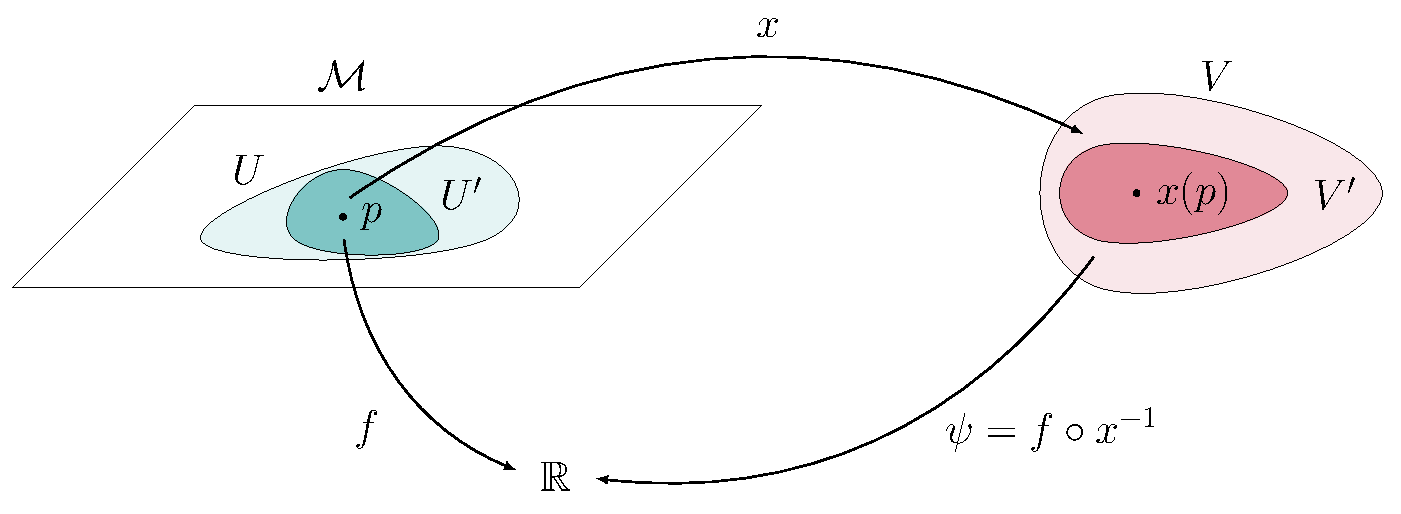
\includegraphics[width=1\linewidth]{figures/tikz/lemma_tangentialvectors.pdf}
\label{img:lemmaDarstellungBasisTPM}
\end{figure}

Nach der Abbildung gilt:
\begin{align}
\psi(u) - \psi(u_0) = \int^1_0 \dv{t} \psi(t u + (1- t) u_0) \dd t
\end{align}
Hierbei ist $u=x(q)$ mit $q \in \mfk$ und $u_0 = x(p)$.
\begin{align}
\psi(u) - \psi(u_0) = \sum_i (u^i- u^i_0) \int^1_0 \underbrace{\dv{\psi}{u'} (t u + (1 - t) u_0) \dd t}_{:= \psi_i (u)}
\end{align}
Setze $f_i = \psi_i \circ x : U \subset \mfk \to \R$.
$f_i$ ist glatt und es gelten folgende Eigenschaften nach Definition:
\begin{itemize}
\item $\psi(u)- \psi(u_0) = \psi(x(q)) - \psi(x(p)) = f(q)- f(p)$
\item $u^i = x^i (q)$
\item $u_0^i = x^i(p)$
\item $\psi_i (u) = \psi_i (x(1)) = f_i(q)$
\end{itemize}
Diese Eigenschaften können wir nun wie folgt verwenden:
\begin{align}
f(q)- f(p) = \sum_{i=1}^n (x_i (q) - x_i (p)) f_i(q)
\end{align}

\begin{align}
\pdv{x_i}\eval_{p} (f) &= \partial_i \underbrace{(f \circ x^{-1})}_{\psi} \big \vert_{x(p)} \\
&= \partial_i \psi \eval_{x(p)}\\
&= \psi_i (x(p)) = f_i (p)
\end{align}
Da $\psi(u) = \psi(u_0) + \sum_i (u^i - u^i_0)\psi_i(u)$
\begin{align}
\Rightarrow \pdv{u_i} \psi \eval_{x(p)} = \psi_i(u) \eval_x(p) = \psi(x(p))
\end{align}
Und somit gilt schließlich $f_i (p) = \pdv{u_i} \eval_p (f)$.
\end{bew}

Nun können wir unseren Beweis fortführen.

\begin{bew}[Satz \ref{satz:BasisTPM} Teil 2] \leavevmode
\begin{align}
v(f) &= v(f(p) + \sum_i (x_i - x_i(p)) f_i) \\
&= v(f(p)) + \sum_i v(x_i - x_i (p) f_i)
\end{align}
Benutze Produktregel
\begin{align}
v(f) &= \sum_i (\underbrace{(x_i (p) - x_i (p)) v(f_i)}_{=0} + \underbrace{v(x_i - x_i (p))}_{=v(x_i)} f_i) \\
&= \sum_i v(x_i) f_i \\
&= \sum_i v(x_i) \pdv{x_i} \eval_p f 
\end{align}
\end{bew}

\begin{satz}[Transformationsregel]
Seien $(x, U)$ und $(\tilde{x}, \tilde{U})$ zwei Karten um $p \in \mfk$.
\begin{figure}[H]
\centering
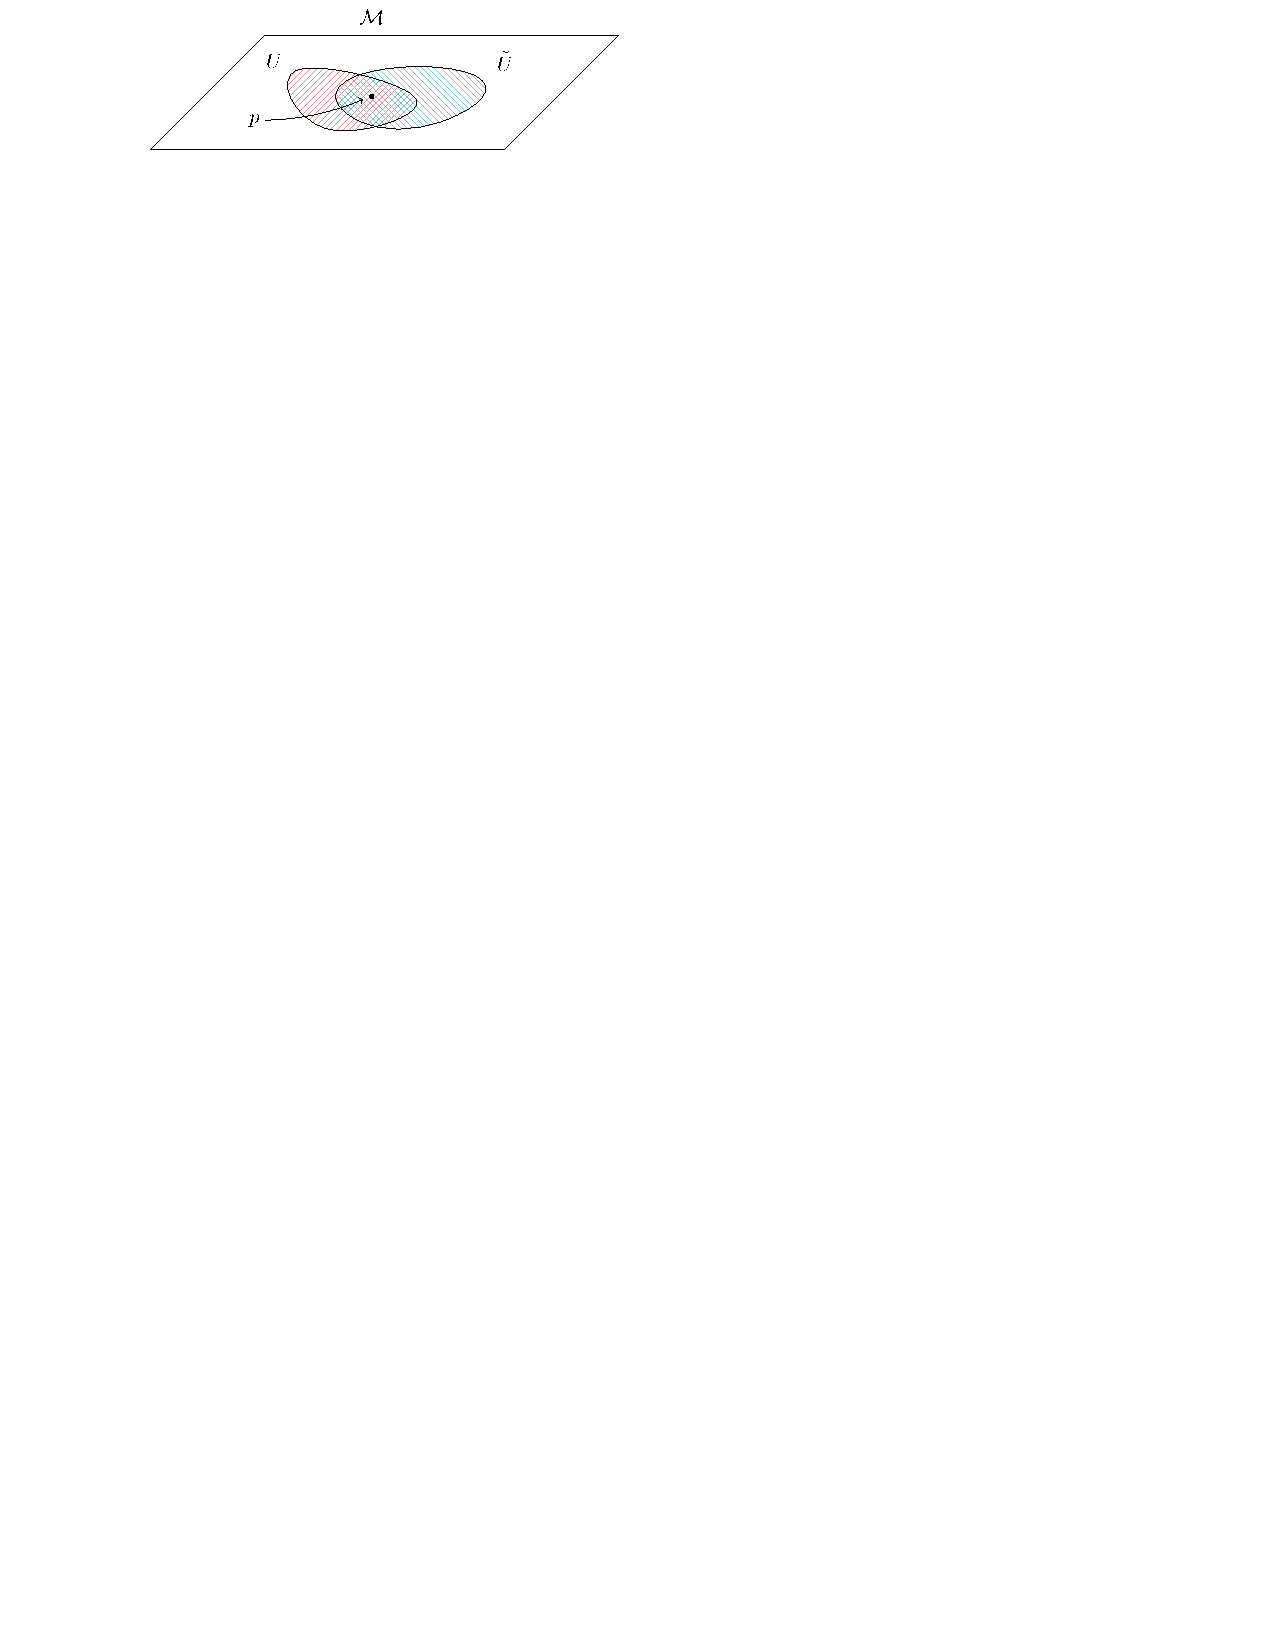
\includegraphics[scale=1.0]{figures/tikz/transformationlaw.pdf}
\label{img:transformationsregel}
\end{figure}  
Dann gilt:
\begin{align}
\pdv{\tilde{x}_i} \eval_p  = \sum_j \underbrace{\pdv{\tilde{x}_i} \eval_p  (x_j)}_{\in \R} \pdv{x_j} \eval_p 
\end{align}
(In der linearen Algebra hatten Transformationen die ähnliche Gestalt: $\tilde{v}_i = \sum_j a_{i j } v_j$)
\end{satz}
\begin{defs}[Differential, Ableitung]
Seien $\mfk$ und $\mfka$ differenzierbare Mannigfaltigkeiten und $f: \mfk \to \mfka$ glatt.
Das \textbf{Differential (Ableitung)} von $f$ in $p$ ist die lineare Abbildung:
\begin{align}
\dd f \eval_p : \tspace{p} &\to T_{f(p)}\mfka \\
v &\mapsto \dd f \eval_p (v),
\end{align}
welche definiert ist durch:
\begin{align}
\underbrace{\dd f \eval_p (v)}_{T_{f(p)}\mfka} \underbrace{(\phi)}_{\in \mathcal{F}(\mfka)} = \underbrace{v(\phi \circ f)}_{\in \mathcal{F}(\mfka)}, \quad \forall \phi \in \mathcal{F}(\mfka)
\end{align}
\end{defs}
Fakt: $\dd f \eval_p$ ist linear.
\begin{satz}[Kettenregel]
\label{satz:Kettenregel}
Seien $f: \mfk \to \mfka$ und $g: \mfka \to \mathcal{P}$ glatte Abbildungen.
Dann gilt:
\begin{align}
\dd (g \circ f) \eval_p = \dd g \eval_{f(p)} \circ \dd f \eval_p
\end{align}
\begin{figure}[H]
\centering
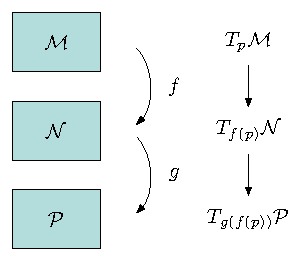
\includegraphics[width=0.45\linewidth]{figures/tikz/chain_rule.pdf}
\label{img:kettenregel}
\end{figure} 
\end{satz}

\begin{bew}[Satz \ref{satz:Kettenregel}] \leavevmode
\begin{align}
\dd (g \circ f) \eval_{p} (v) (\phi) &= v(\phi \circ g \circ f) \\
&= \dd f \eval_p (v)(\phi \circ g) \\
&= \dd g \eval_{f(p)} \circ \dd f \eval_p (v) (\phi)
\end{align}
\end{bew}

\begin{satz}
Sei $f: \mfk \to \mfka$ glatt und sei $(x, U)$ eine Karte von $\mfk$ um $p$ und $(y, V)$ eine Karte von $\mfka$ um $p$.
Setze $f_j = y_j \circ f$ mit $f_j : \mfk \to \R$, dann gilt:
\begin{align}
\underbrace{\dd f \eval_p ( \pdv{x_i} \eval_p)}_{\in T_{f(p)}\mfk} = \sum_j \underbrace{\pdv{x_i}\eval_p (f_j)}_{\in \R} \underbrace{\pdv{y_j} \eval_{f(p)}}_{\in T_{f(p)}\mfka}
\end{align}
\end{satz}

\begin{defs}[regulärer Wert/Punkt, Submersion, Immersion] 
Sei $f: \mfk \to \mfka$ glatt und es gelte $\dim\mfk=m$, $\dim{\mfka} = n$.
\begin{enumerate}
\item $\rang f$ in $p$ ist $\rang \dd f \big \vert_p $.
\item $p\in\mfk$ heißt regulärer Punkt ($\in\mfk$)  $\Leftrightarrow \rang\dd f \eval_p=\dim\mfka$.
\item $q\in\mfka$ heißt reguläreer Wert ($\in\mfka$) $\Leftrightarrow \forall p \in f	^{-1}(q)$ sind reguläre Punkte.
\item $f$ heißt Submersion $\Leftrightarrow$ $f$ surjektiv und alle $p\in\mfk$ sind reguläre Punkte.
\item $f$ heißt Immersion $\Leftrightarrow$ $\dd f \eval_p$ injektiv für alle $p \in \mfk$
\end{enumerate}
\end{defs}

\begin{satz}[Umkehrsatz]
\label{satz:Umkehrsatz}
Sei $f: \mfk \to \mfka$ glatt. 
Sei $\dd f \eval_p : \tspace{p} \to T_{f(p)}\mfka$ ein Isomorphismus,
dann existiert eine Umgebung $U$ um $p$ und eine Umgebung $U'$ um $f(p)$, so dass
\begin{align}
f\eval_U : U \to U'
\end{align}
ein Diffeomorphismus ist.
\begin{figure}[H]
\centering
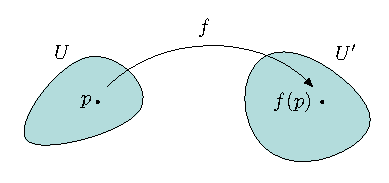
\includegraphics[width=0.5\linewidth]{figures/tikz/inverse_function_theorem.pdf}
\label{img:umkehrsatz}
\end{figure} 
\end{satz}

\begin{bew}[Satz \ref{satz:Umkehrsatz}] \leavevmode
Nutze Karten um dies auf den euklidischen Fall zu führen.

\begin{align}
\begin{xy}
  \xymatrix@=0.25\linewidth{
      \mfk \ar[r]^f \ar[d]_x    &   \mfka \ar[d]^y \\
      V\subseteq \R^m \ar[r]_\phi             &   V\subseteq \R^m    
  }
\end{xy}
\end{align}

Seien $(x, U)$ und $(y, U')$ Karten von $\mfk$ und $\mfka$ um $p$ und $f(p)$.
Ohne Beschränkung der Allgemeinheit gilt: $f(U) \subset U'$.
Dann ist $\phi$ eine glatte Abbildung deren Differential $\dd \phi \eval_{x(p)}$ invertierbar ist.
Umkehrsatz im $\rn$ auf $\phi$ anwenden:
Es existieren Umgebungen $\hat{V}$ von $x(p)$ und $\hat{V}'$ von $y(f(p)) = \phi(x(p))$, so dass
$\hat{\phi}\eval_{\hat{V}}$ ein Diffeomorphismus ist.
Dann ist
\begin{align}
f\eval_{x^{-1}(\hat{V})}: x^{-1}(\hat{V}) \to y^{-1}(\hat{V}')
\end{align}
ein Diffeomorphismus.
\begin{align}
\phi = y \circ f \circ x^{-1} \Rightarrow f = y^{-1} \circ \phi \circ x
\end{align}
\end{bew}


\begin{satz}[Satz über implizite Funtionen]
\label{satz:Satz über implizite Funtionen}
\end{satz}
Sei $f: \mfk \to \mfka$ glatt und es gelte $\dim\mfk=m$, $\dim{\mfka} = n$.
\begin{enumerate}
\item Sei $\rang_p f = r$ und $v \in V$ und $V \subseteq \R^m$. 
Dann existiert zu jeder Karte  $(y, U')$ um $f(p)$ eine Karte $(x, U)$ um $p$, so dass
\begin{align}
y \circ f \circ x^{-1}(v_1, \dots, v_m) = (v_1, \dots, v_r, \phi_{r+1}(v), \dots, \phi_n(v)).
\end{align}
Falls $y(f(p))=0$, so kann man $x$ so wählen, dass $x(p)=0$ und $\phi_j (0) = 0$ ($\forall j > r$).

\item Sei $\rang f = r$ auf einer Umgebung von $p$.
Dann gibt es Karten $(x, U)$, $(y, U')$, so dass 
\begin{align}
y\circ f \circ x^{-1} (v_1, \dots, v_m).
\end{align}

\end{enumerate}
\begin{bew}[Satz \ref{satz:Satz über implizite Funtionen} Teil 1]
Wähle Karten und modifiziere diese geschickt.
Sei $(y, U')$ eine Karte von $\mfka$ um $f(p)$.
Sei $(\hat{x}, U)$ eine Karte von $\mfk$ um $p$ mit $\hat{x}(p) = 0$.
Setze 
\begin{align}
\hat{A} = (\hat{A})_{i j} = (\partial_i \hat{\phi}_j),
\end{align}
mit $\phi = y \circ f \circ x^{-1}$.
Da $\rang_p f = r$, können wir ohne Beschränkung der Allgemeinheit annehmen, dass
\begin{align}
\det \tilde{A} \neq 0.
\end{align}
Wobei hier nun $\tilde{A} = (\hat{A}_{i j})_{1 \leq i \leq r}$.
Setze 
\begin{align}
x_i = \left\{
\begin{array}{ll}
y_i \circ f & \quad 1 \leq i \leq r \\
\hat{x}_i & \textrm{falls} \ r+1 \leq i \leq n \\
\end{array}
\right. 
\end{align}
Dann gilt $x(p)=0$ und 
\begin{align}
\partial_i (x_j \circ \hat{x}^{-1})(0) = 
\left(\begin{matrix}
\partial_i \hat{\phi}_j (0) & \star \\ 
0 & \mathds{1}
\end{matrix} \right) .
\end{align}
Daraus folgt, dass $\rang x = m = \dim \mfk$ im Punkt $p$.
Mit Hilfe des Umkehrsatzes folgt, dass $x$ ein lokaler Diffeomorphismus ist 
und eine Umgebung $U$ um den Punkt $p$ existiert und eine Umbegungen $V$ von $0$ in $\rn$, 
sodass $x: \mfk \to V$ eine Karte ist und
\begin{align}
\phi (v_1, \dots, v_m) &= y \circ f \circ x^{-1}(v_1, \dots, v_m) \\
&= (v_1, \dots, v_r, \phi_{r+1}(v), \dots, \phi_m (v)).
\end{align}
Wobei $\phi_k$ glatt auf $U'$ sind mit $\phi_i(0)=0$. 
Betrachte die Jacobi-Matrix:
\begin{align}
A_{i j} = (\partial _i \phi_j )_{i j} = \begin{pmatrix}
\mathds{1} & 0 \\ 
\star & \partial_i \phi_j
\end{pmatrix} 
\end{align}
Da $\rang \phi = r$ in einer Umgebung von $U=0$ hat folgt:
\begin{align}
\partial_i \phi_j = 0 \quad \forall i, j > r.
\end{align}
\end{bew}

\begin{kor}
Sei $f: \mfk \to \mfka$ mit $\dim \mfk = m$ und $\dim \mfka = n$ glatt, dann gilt:
\begin{enumerate}
\item Sei $q \in \mfka$ ein regulärer Wert, so ist 
\begin{align}
\mathcal{H} = f^{-1}(q) = \{ p \in \mfk (f(p))=q \}
\end{align}
eine Untermannigfaltigkeit der Dimension $m-n$.
\item Sei $f$ linear in einer Umgebung von $\mathcal{H} = f^{-1}(q)$ vom $\rang$ $r$, so ist $\mathcal{H}$ eine Untermannigfaltigkeit der Dimension $m-r$.
Der Tangentialraum $T_p \mathcal{H}$ ist isomorph zu
\begin{align}
\ker \dd f \eval_p \subseteq \tspace{p}, \quad \forall p \in \mathcal{H}.
\end{align}
\end{enumerate} 
\end{kor}